%!TEX root=paper.tex

\newpage
% \section{How Do Students Improve Their Vocabulary?}
% \section{How Does The System Help Students Improve Their Vocabulary?}
% \section{What Is The Impact of the System on the Learner Vocabulary?}
% \section{Does The Vocabulary of the Learners Improve?}
\section{Do Students Improve Their Vocabulary?}

  The value of extensive reading can be found, besides the new words that are learned, in the strengthening of the knowledge of the existing words, increased fluency, and increased grammar knowledge. Some of these benefits can be reliably measured only after a time longer than our deployment \cite{renadya07-power}. 

  However, since our system combines free reading with vocabulary exercises and tracks all word interactions, by analyzing the learner interaction with the reader and the exercises, we can provide a glimpse into two measures of progress visible after one month of usage: increasing confidence about words and learning new words. 

   \begin{figure}[h!]
  \centering
    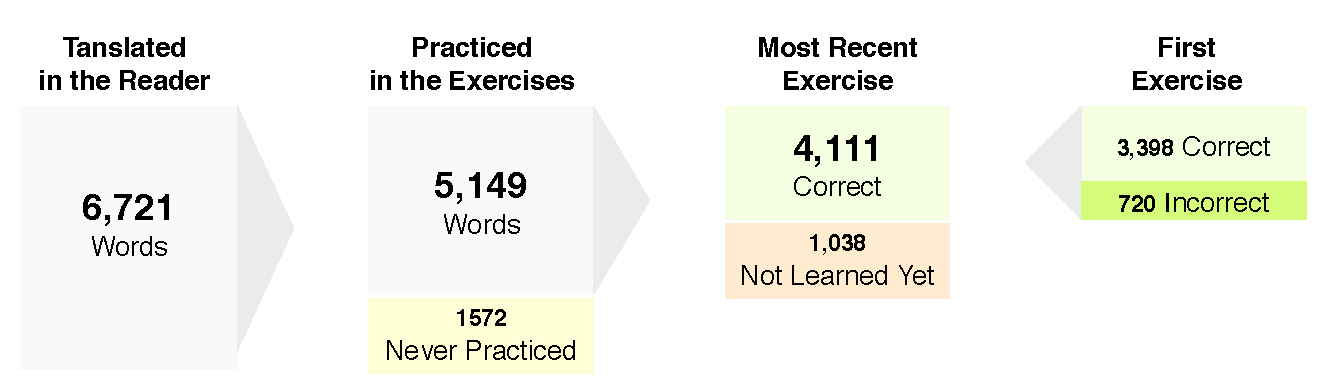
\includegraphics[width=0.87\columnwidth]{figures/word-learning-flow.pdf}
    \caption{Word encounters in the Reader and Exercises}
    \label{fig:word_learning_flow}
  \end{figure}

  Figure \ref{fig:word_learning_flow} summarizes visually the interactions of the students with words in the reader and the exercises parts of the system. The figure is based on the analysis of the user interaction database and shows that: 

  \begin{itemize}
    \item From the 6,721 words that were looked up in the reader, 5,149 were used in the exercises platform. Since the learners requested a translation for these words we can assume that they were not known to the readers or at least the readers were unsure about their meaning. 

    \item More than 1,500 words were not practiced in the exercises. 
    Some did not get their turn to be scheduled by the algorithm and others were not presented because the system deemed them not fit for study (cf. Vocabulary Recommender, p.3). 
    % Given that not all the words can be practiced, this is an argument for prioritizing the words that the students are presented with in the exercises.

    \item For 4,111 words (80\% of all the words present in exercises) the learners were able to correctly identify the meaning in the last associated exercise. Out of these: 

    \begin{itemize}
      \item 720 words (14\% of all the words in exercises) were wrong during their first exercise interaction but were correct in the final one. These {\bf 720 words are likely to be learned via the exercises} by the sixty students in our study. They represent 10.75\% of all the words that the students translated in the reader.

      \item 3,391 words (66\% of all the words in exercises) were recognized already for the first time in the exercises. These are {\bf likely to be words for which the knowledge was strengthened by using the system}: the students were unsure when encountering them initially in the reader but eventually recognized their meaning when encountering them later in the exercises\footnote{It could also be that the students learned them after the first encounter in the text, but we keep the more conservative hypothesis}. 
    \end{itemize}

  \item For 1,038 words (20\% of all the words present in exercises) the outcome of the final exercise that involved them showed an incorrect answer. Thus we can assume that they were {\bf still not learned at the end of the experimental period}.

  \end{itemize}

% \end{added}
